\documentclass[../main.tex]{subfiles}
\graphicspath{{\subfix{../images/}}}
\usepackage{subfiles}
\usepackage{subfig}

\begin{document}
    \section{Time Series Forecasting}
        In this comprehensive section, we will delve deeper into the fascinating world of time series forecasting. Our exploration will encompass an extensive review of the various techniques available, allowing us to gain a comprehensive understanding of each approach's particularities and guiding principles. To ensure a well-rounded discussion, we will commence with an overview of traditional forecasting methods, exploring their strengths and limitations. Subsequently, we will progress to more advanced techniques that harness the power of deep learning, leveraging its capabilities for enhanced prediction accuracy. \par

        Throughout this section, we will enrich our understanding of these forecasting techniques by presenting a compelling case study. The case study will focus on data collected from Lawson female workers, comprising a diverse range of variables, including heart rate (HR), movement patterns, and temperature. By utilizing this real-world dataset, we will illustrate how these forecasting methods can be effectively applied in practice, elucidating their practical implications and showcasing their performance on complex biosignal data. The dataset measures activity as the root of the sum squared of the acceleration in the three axis (x, y and z) subtracted by one to disregard the gravitational acceleration component, as shown in equation \ref{eq:activity}. All the values were actually not measured in equally spaced intervals, but instead at every heartbeat, so an averaging of the values at every minute was taken for the heart rate, and the maximum activity in the interval was taken. Figure \ref{fig:hr_activity} shows the variation of the activity and heart rate as a function of time for the dataset at hand. \par

        \begin{equation}
            \label{eq:activity}
            Activity = \sqrt{a_x^2+a_y^2+a_z^2}-1
        \end{equation}

        \begin{figure}[h]
            \begin{center}
            \centering
            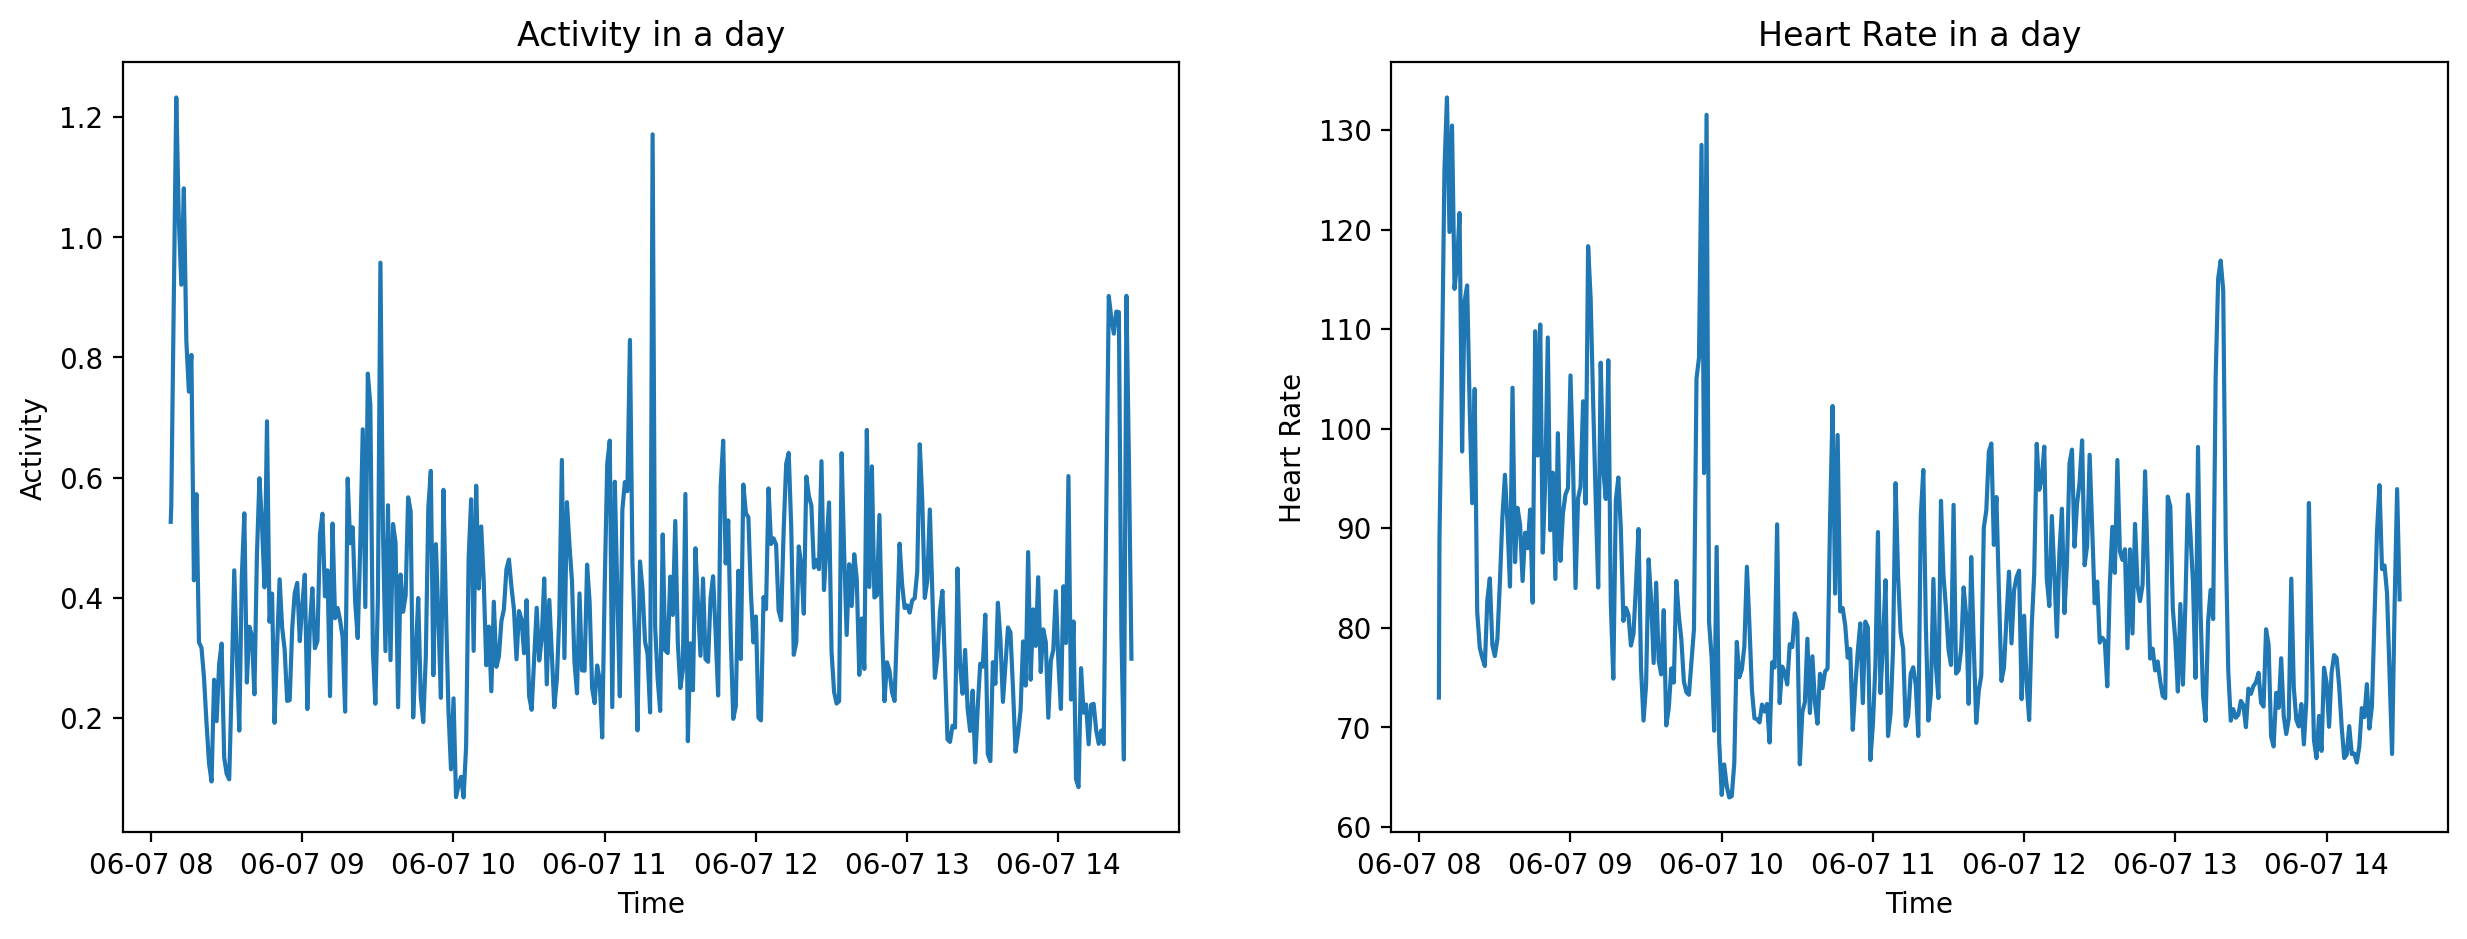
\includegraphics[width={\columnwidth}]{images/heart_rate_activity.png}
            \caption{Plot of the measured Heart Rate and Activity for a worker in a given day as a function of time.}
            \label{fig:hr_activity}
            \end{center}
        \end{figure}

        By integrating theoretical discussions, practical examples, and case studies, this section aims to equip readers with a holistic understanding of time series forecasting techniques. Whether you are a researcher, data scientist, or healthcare professional, this comprehensive exploration will empower you to confidently select and apply the most suitable forecasting approach for your specific problem domain, unlocking the potential to make accurate predictions and informed decisions based on biosignal time series data.\par

        \subfile{Subsections/traditional_techniques}
        \subfile{Subsections/deep_learning}

\end{document}